\chapter{Oracle Aplication Express}


\section{Menentukan Tabel}
Dalam hal ini sebelum membuat aplikasi Sistem Akademik terlebih dahulu menentukan 
tabel apa saja yang akan dibutuhkan yaitu (Mahasiswa, Dosen, Matakuliah, Nilai dan Jadwal) lalu
merancang atribut atribut apa saja yang dibutuhkan dalam setiap tabel tersebut. Berikut merupakan rancangan 
dari tabel-tabel yang akan berelasi.
\begin{enumerate}
\item[1]Rancangan Database

\begin{figure}[!htbp]

    \begin{center}
        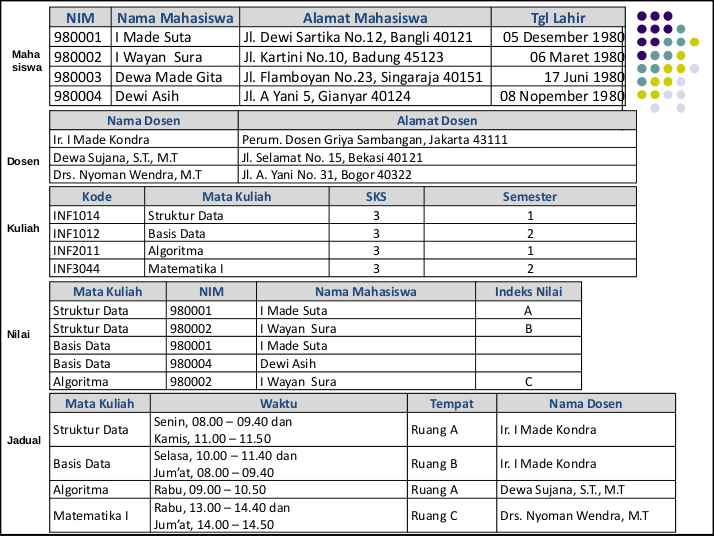
\includegraphics[scale=0.6]{figures/tabelMhs.png}
        \caption{\textit{Rancangan Database}}
        \end{center}   
        \end{figure}
        \begin{figure}[!htbp]

    \section{Membuat Aplikasi dengan Apex}
    Sebelum membuat aplikasi di oracle apex sebaliknya terlebih dahulu
    membuat tabel-tabel yang sudah dibuat sebelumnya kedalam data exel dengan format csc
    setelah itu Create Aplication lalu pilih From A File untuk mengimport data exel yang sudah
    dibuat sebelumnya seperti gambar dibawah ini


    \begin{center}
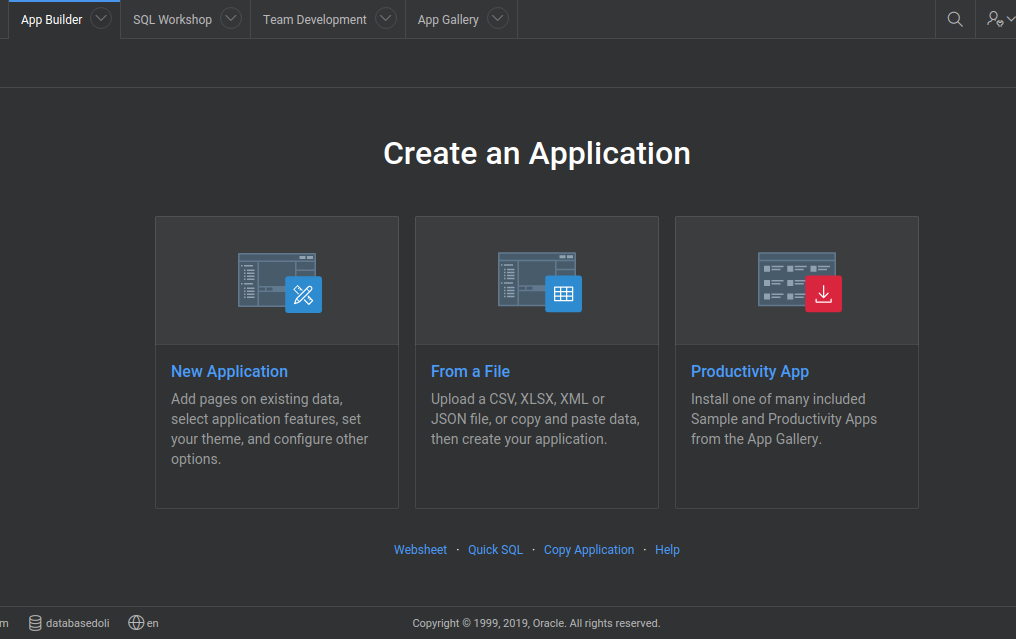
\includegraphics[scale=0.4]{figures/createAppFromfile.png}
    \caption{\textit{Oracle Apex App Builder}}
        \end{center}
\label{gambar}
\end{figure}

\begin{figure}


    \section{Load Data Exel}
    Masukan semua data exel yang sudah di buat didalam exel secara bergiliran
    setiap sheetnya lalu masukkan nama tabel dan save configurasi sampai semua 
    tabel masuk 
    \begin{center}
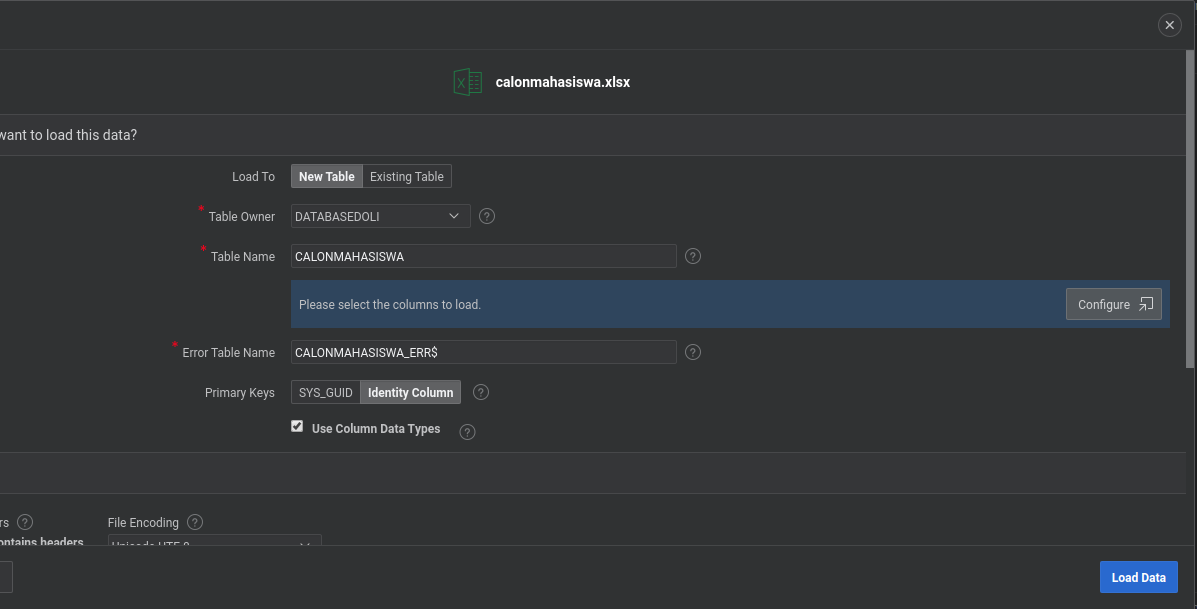
\includegraphics[scale=0.3]{figures/dataexel.png}
    \caption{\textit{Load Data.}}
        \end{center}
\label{gambar}
\end{figure}



\begin{figure}
\section{Konfigurasi Tabel}
Setelah selesai me-load semua tabel maka setiap tabel akan tampil seperti
dibawah ini disini setiap tabel database bisa manipulasi, dibawah ini merupakan tabel Mahasiswa
yang dibuat melalui exel sebelumnya.
    \begin{center}
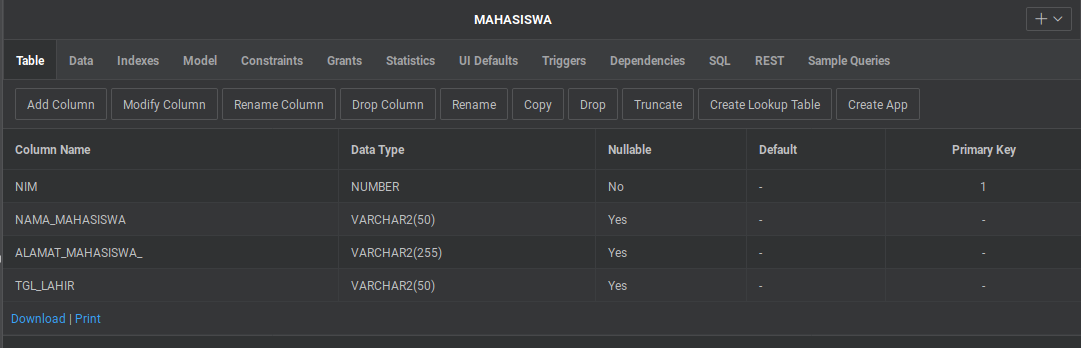
\includegraphics[scale=0.4]{figures/mhsTabel.png}
    \caption{\textit{Konfigurasi Tabel}}
        \end{center}
\label{gambar}
\end{figure}

\begin{figure}

\section{Normalisasi Tabel Datase}
Untuk membuat relasi antar tabel terlebih dahulu men-set field (nim) sebagai
 Primary Key dari tabel(Mahasiswa, Dosen, Matakuliah)
berguna sebagai key dari tabel tersebut (Lakukan sebaliknya pada tabel Dosen
dan Matakuliah)

    \begin{center}
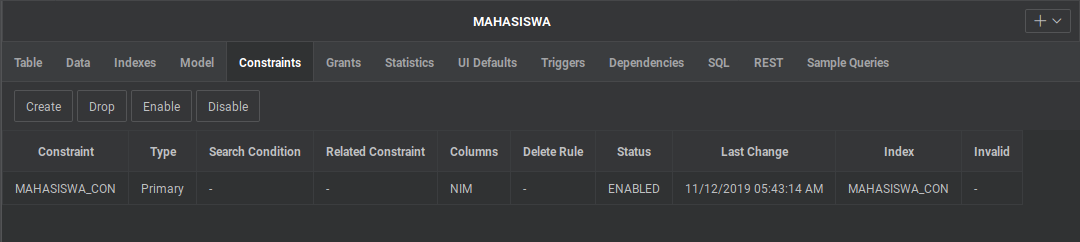
\includegraphics[scale=0.4]{figures/primaryKey.png}
    \caption{\textit{Primary Key}}
        \end{center}
\label{gambar}
\end{figure}

\begin{figure}
\section{Foreign Key}
Dibawah ini kita membuat relasi antara (Tabel Mahasiswa dan Tabel Nilai) dengan men-set (nim) yang terdapat pada
tabel Nilai sebagai foreign key dan relasi antara (Tabel Dosen dan Jadwal) dengan men-set (nik) yang terdapat pada
tabel jadwal sebagai foreign key
    \begin{center}
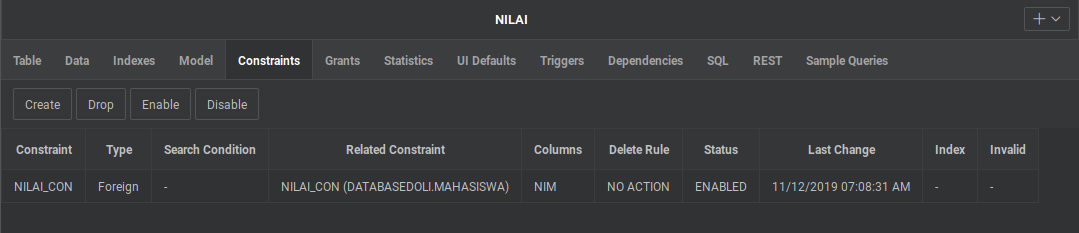
\includegraphics[scale=0.4]{figures/foreignKey.png}
    \caption{\textit{Foreign Key}}
        \end{center}
\label{gambar}
\end{figure}

\begin{figure}
\section{Create Aplication}

Setelah semua selesai kita akan kembali ke halaman utama dari oracle apex untuk membuat aplikasi akademik
sederhana dengan menggunakan kelima tabel yang sudah berelasi sebelumnya
yang ditampilkan sebagai berikut

    \begin{center}
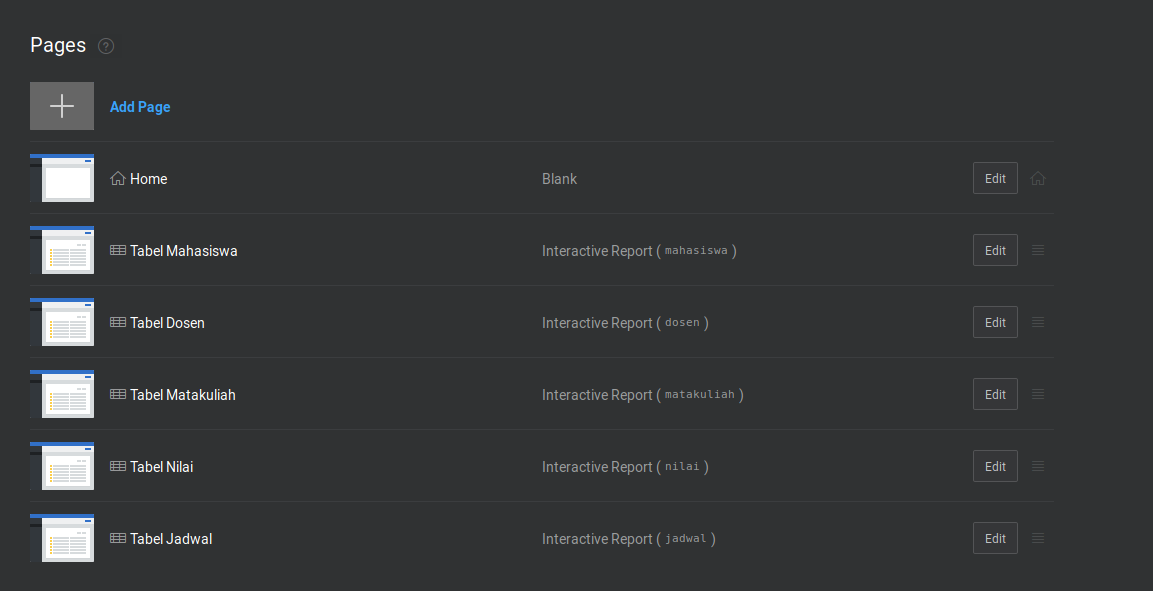
\includegraphics[scale=0.4]{figures/tugasdb3_7.png}
    \caption{\textit{Create Aplication}}
        \end{center}
\label{gambar}
\end{figure}

\begin{figure}
    \section{Halaman Login}
    
    Setelah semua selesai kita akan kembali ke halaman utama dari oracle apex untuk membuat aplikasi akademik
    sederhana dengan menggunakan kelima tabel yang sudah berelasi sebelumnya
    yang ditampilkan sebagai berikut dengan password (pemograman2) 
    
        \begin{center}
    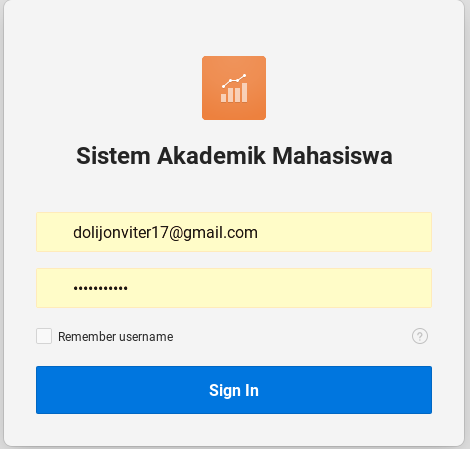
\includegraphics[scale=0.5]{figures/tugasdb3_8.png}
        \caption{\textit{Halaman Login}}
            \end{center}
    \label{gambar}
    \end{figure}

    \begin{figure}
        \section{Sistem Akademik Mahasiswa}
        (Link Aplikasi berada pada file url.ext)
            \begin{center}
        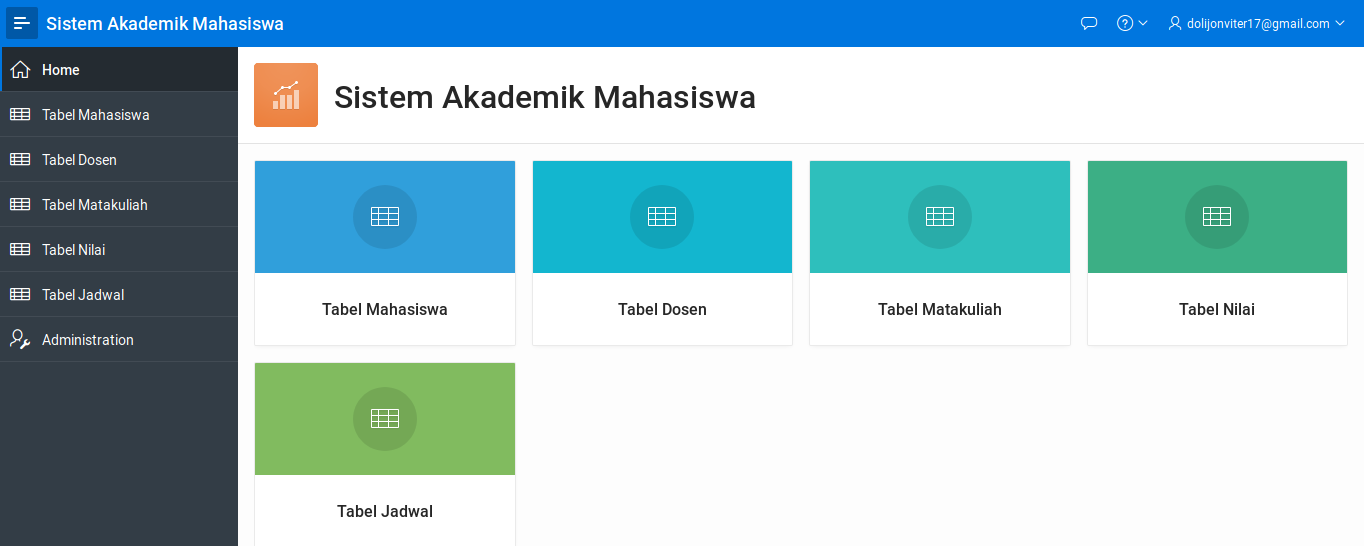
\includegraphics[scale=0.3]{figures/hasilAkhir.png}
            \caption{\textit{Halaman Login}}
                \end{center}
        \label{gambar}
        \end{figure}

\end{enumerate}




    

